\section{Survey Sections} \label{sec:survey}
Now that AIA, assurances, trust, and TRBs have been defined we are ready to being the survey regarding what assurances exist, and how to proceed with their design. The obvious place to start is with those researchers who have formally addressed the topic of trust between humans and AIAs of some form. Here we consider formal treatment of trust to be those who acknowledge a human trust model and who perform experiments that attempt to measure the effect of assurances on trust.

However, this leaves out a much larger body of those who have informally considered trust in their work. In this case I define informal to mean those who only reference the nebulous idea of trust, and who do not actually perform experiments to verify that assurances actually do affect trust.

Conversely, much of the formal research has focused on implicit assurances. This is likely due to the focus on analyzing the effect of autonomous systems on trust and not on designing systems for trust. However as seen by a large spike in interest in `interpretable', and `explainable' AIAs in government, academic, and public circles, there is a large need for designed assurances.

\begin{figure}[htbp]
    \centering
    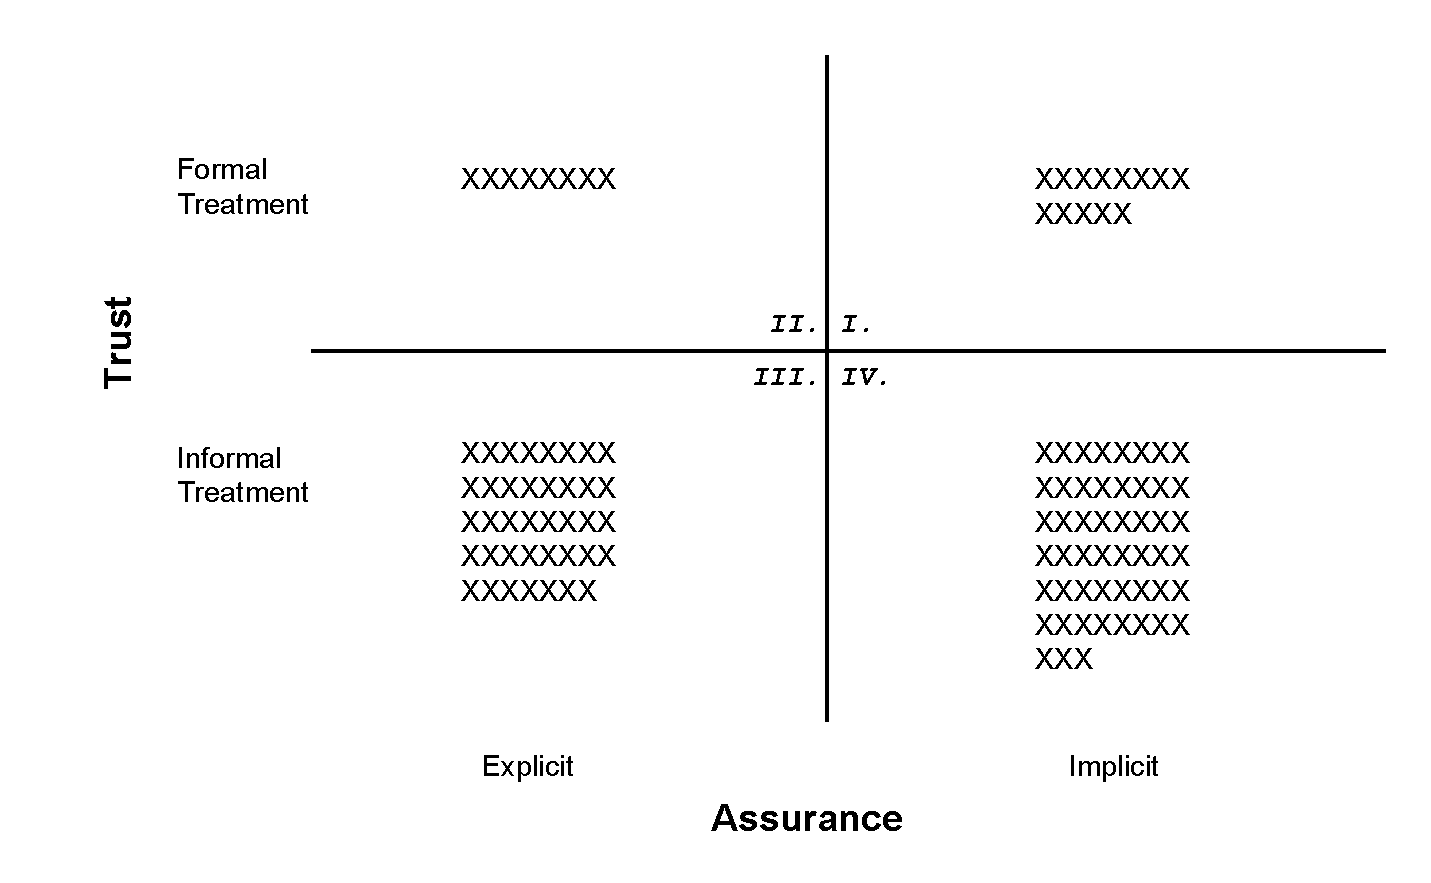
\includegraphics[width=0.6\textwidth]{Figures/Trust_vs_Assurance_Intention.pdf}
    \caption{Figure depicting how many papers that consider trust formally/informally consider intentional/unintentional assurances, \textbf{need to put actual data here, if it is a useful figure, for now the data is approximate from my memory}}
    \label{fig:trust_assurance_intention}
\end{figure}

The remainder of this survey will focus on surveying the assurance research in the formal/informal, explicit/implicit plane. Figure \ref{fig:trust_assurance_intention} shows the number of papers considered in this survey that lay in each quadrant of that plane. The quadrants are defined as:

\begin{itemize}
    \item Quadrant I. (implicit, formal) -- Use human experiments, consider a trust model, assurances are implicit (i.e. those who care about trust, but aren't designing assurance algorithms)
    \item Quadrant II. (explicit, formal) -- Use human experiments, consider a trust model, assurances are explicit (i.e. those who formally acknowledge trust from an AIA, and design assurances to affect it)
    \item Quadrant III. (explicit, informal) -- No human experiments, reference trust (or interpretability, etc..), proposed assurances are explicit (i.e. those who know that ``trust'' is important, but really just present their opinion about an algorithm that might be an assurance)
    \item Quadrant IV. (implicit, informal) -- don't reference trust, designed properties of AIA for better performance, typically reference some of the trust components such as predictability, stability, verification, but only in the context of the designer being happy.(i.e. those whose work is relevant for assurances, but they don't know it)
\end{itemize}

It is clear that much of the research that is relevant has occurred in the informal half of the plane. The aim, in order to satisfy the need for trust in AIAs, is to create more research in Quadrant II. This would mean that assurances have been formally and explicitly designed to affect user's trust. One key observation, is that there is plenty of opportunity to `move' research from Quadrants I., III., and IV. to Quadrant II. In essence this would be taking proposed methods and putting them to the test using a formal understanding of trust and appropriately designed experiments.

\subsection{Intentional and Unintentional Assurances}
    There seems to be quite a large disparity of the kinds of assurances studied by the formal and informal trust groups, as depicted in Figure \ref{fig:trust_assurance_intention}.  This is most likely due to the differing interests and skill sets. Those studying unintentional assurances seem to be more interested in investigating the human-AIA relationship. On the other hand those investigating the effect of intentional assurances are more interested in making algorithms.
    
    This figure clearly shows that there is a large space for researchers who study intentional assurances within a formal trust framework. To state the idea more clearly, this would involve actively designing assurances based on the AIA capability, and the assurance classes, and then validating these assurances in designed experiments.

    \textbf{add more stuff \ldots}


\subsection{Other stuff \ldots}
